\chapter{捐赠信息披露对开发者活动的影响}
%%====================================================================

本章围绕第一个研究问题展开：外部非盈利基金会的两种捐赠信息披露方式，如何分别及交互地影响开发者活动？以 Bitcoin Brink 基金会（以下简称”Brink”）在2022—2023年间的真实披露事件为研究对象，本章从理论层面整合期望理论与期望失验理论，构建了一个统一解释非定向披露正向主效应、定向披露正向主效应以及两者间负向交互效应的分析框架。实证层面，本章借助固定效应面板模型与两阶段最小二乘法，基于169,785个开发者—周观测单元对三组假设加以检验；机制层面，则通过两组开发者异质性分析，揭示信息激励效应的作用边界与强化条件。

全章结构安排如下：第~\ref{sec:research-scene-1} 节介绍 Bitcoin Brink 研究场景及两类披露的运作机制；第~\ref{sec:hypotheses-1} 节基于理论推演提出研究假设；第~\ref{sec:data-1} 节说明数据来源、样本构建与变量定义；第~\ref{sec:model-1} 节阐述计量模型设定与识别策略；第~\ref{sec:results-1} 节呈现主效应估计结果；第~\ref{sec:robust-1} 节报告稳健性检验；第~\ref{sec:mechanism-1} 节开展机制分析；第~\ref{sec:summary-1} 节总结本章主要发现及理论贡献。

\section{研究场景：Bitcoin Brink 生态}
\label{sec:research-scene-1}

\subsection{Brink 基金会简介}

Bitcoin Brink（以下简称”Brink”）成立于2020年，
是当前规模最大、专注于比特币核心协议开发的非营利性资助机构。
不同于 GitHub Sponsors 等点对点赞助机制，Brink 采用集中式众筹模式——
面向个人捐赠者和机构投资者募集资金，经严格申请与审核流程后，
将资助名额授予比特币开源社区中贡献突出的全职开发者，
为其提供可持续的薪资支持。

Brink 的成立源于一个长期存在的结构性隐患：比特币核心开发高度依赖少数全身心投入的志愿者，一旦这些开发者因经济压力减少投入，整个网络的安全性与发展节奏将面临系统性风险。比特币核心代码库（\texttt{bitcoin/bitcoin}）是比特币网络的权威实现，其质量与安全性直接关系到数千亿美元资产的存储与转移。但该关键基础设施长期以来几乎完全依赖自愿性无偿贡献维持，由此造成对极少数全职核心开发者的高度依赖——据估计，长期活跃的核心维护者不足二十人。这种”关键少数”结构意味着，任何一位核心开发者的退出都可能对项目进展造成显著冲击。Brink 正是在此背景下设立的，定位为比特币开发基础设施的”社会保障网络”：通过提供稳定经济保障，降低优质开发者离开社区的概率，保障比特币基础设施的可持续迭代。

Overney 等（2020）\cite{overney2020not} 对开源社区捐赠模式的系统研究表明，点对点捐赠模式（如直接向个人开发者捐款）存在明显的”马太效应”——知名度高的开发者获得的捐款远多于贡献水平相当但知名度较低的同行。Brink 的集中式筛选与分配模式在一定程度上纠正了信息不对称所导致的资源分配失衡，同时也形成了本研究所关注的特殊信息披露结构。

Brink 的运营从捐款募集到资助落地，经历清晰可追踪的两阶段信息披露过程
（图~\ref{fig:brink-flow}）。这一双阶段结构为本研究提供了独特的识别机会。

\begin{figure}[htbp]
    \centering
    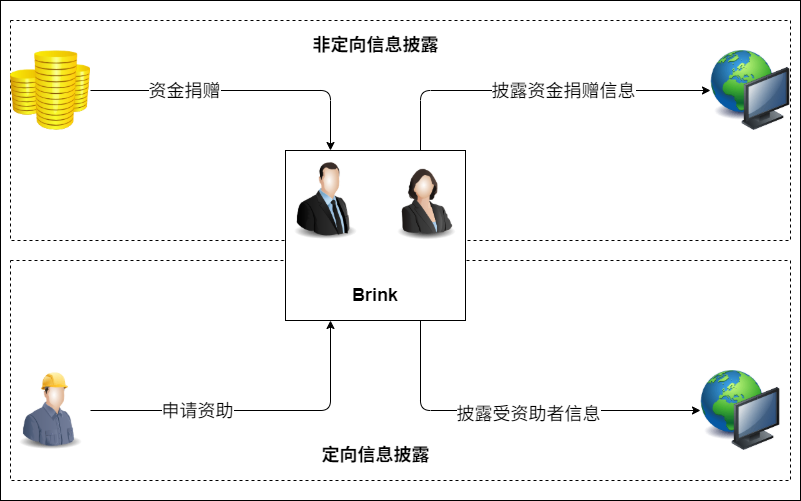
\includegraphics[width=0.62\textwidth]{figures/bitcoinbrink_operation.png}
    \caption{Brink 捐赠信息披露流程}
    \label{fig:brink-flow}
\end{figure}

\subsection{非定向披露的运作机制}

Brink 每完成一笔捐款的接收与确认，便在其官方 X（原 Twitter）账号 @bitcoinbrink 发布捐赠公告。公告内容一般包含捐赠方名称、捐款金额及对捐赠方的公开致谢，但不涉及资金用途的任何具体说明——即无法从公告中判断该笔资金将最终资助哪位开发者。本研究观测期（2022年1月至2023年12月）内，Brink 共发布此类非定向披露公告19次，其中15次明确披露了具体捐款金额，单笔金额从数千美元到500万美元不等，跨期变动幅度相当大。非定向披露的典型形式为 X 平台上的简短推文，包含以下要素：捐赠方名称或代号、捐款金额（以美元或比特币计）、对捐赠方的致谢语，以及 Brink 对持续推动比特币核心开发的承诺声明。这类推文信息密度较低，内容高度标准化，不涉及具体资助用途或受助候选人。图~\ref{fig:untargeted-example} 所示为一条典型的非定向披露推文：Brink 宣布收到来自 @jack 与 \#startsmall 的500万美元捐款承诺，公告仅涉及捐款金额和致谢，未说明资金将定向资助任何特定开发者。

\begin{figure}[htbp]
    \centering
    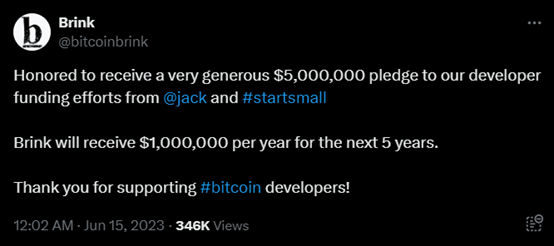
\includegraphics[width=0.72\textwidth]{figures/untargeted_example.png}
    \caption{非定向披露示例：Brink X 平台捐款公告（2023年6月15日）}
    \label{fig:untargeted-example}
\end{figure}

就信息传播路径而言，X 平台的公告面向所有公开关注者，不区分身份与贡献层级。Brink 生态中从事开发工作的1600余名开发者均有机会第一时间获取该信息。公告并未指定受益方，因而每位开发者在获知”有大额捐款注入”时，都可合理地将自己纳入未来受益者的范畴。Kobayakawa 等（2020）\cite{kobayakawa2020impact} 的研究已表明，加密货币市场的资本规模与开源开发活动之间存在正向关联，Brink 的捐款公告恰恰是将加密货币生态的资本流动与开源开发者激励感知直接联结起来的传播节点。这种”普惠性”信息结构，构成非定向披露区别于其他激励机制的核心特征。

从期望理论视角看，非定向披露至少通过两条心理路径影响开发者行为意愿。其一为效价路径：捐款公告向外界传递了”Brink 掌握充足资金，有能力资助更多开发者”的积极信号，提升开发者对潜在奖励价值的主观评估。其二为期望路径：公告释放的资金实力信号强化了开发者对”当前活动行为能够获得回报”这一预期的信心。两条路径共同作用下，非定向披露有望在短期内促进活动参与的增加。该机制实质上类似于众筹平台的资金积累公示效应——Wang 等（2022）\cite{wang2022monetary} 在分析货币激励与知识溢出时即指出，公开的资金规模信息能够通过期望路径有效激励潜在贡献者的参与投入。

\subsection{定向披露的运作机制}

定向披露与非定向披露的性质截然不同，它发生在 Brink 完成内部审核并正式确定受资助开发者之后。Brink 通过在官方网站（\url{https://brink.dev}）更新受资助者页面，公开列出获批开发者的 GitHub 用户名、资助开始时间及资助期限。这类披露指向性明确：信息内容从”谁捐了多少钱”变为”谁通过审核、谁获得了资助”，标志着抽象激励预期向可观察的分配事实的转化。

在本研究的观测窗口内，Brink 共进行了5次定向披露，受资助开发者及公告时间汇总如表~\ref{tab:grantees} 所示。

\begin{table}[htbp]
    \centering
    \caption{Brink 受资助开发者名单（2022年1月—2023年12月）}
    \label{tab:grantees}
    \begin{tabularx}{\textwidth}{p{2.8cm}Xp{4.5cm}}
        \toprule
        披露日期 & 受资助开发者（GitHub 用户名） & 说明 \\
        \midrule
        2022年4月4日  & 0xB10C、vincenzopalazzo、dergoegge、brunoerg & 本轮共资助4名开发者，规模最大 \\
        2022年5月13日 & fanquake & 单独资助 \\
        2022年6月30日 & adiabat   & 单独资助 \\
        2022年7月29日 & stickies-v & 单独资助 \\
        2023年5月4日  & fjahr      & 单独资助 \\
        \bottomrule
    \end{tabularx}
\end{table}

图~\ref{fig:targeted-example} 展示了规模最大的一次定向披露（2022年4月4日）的官方公告页面截图。Brink 在其中明确列出4名获批开发者的姓名及比特币开发背景，信息的指向性与权威性同非定向披露形成鲜明对照。

\begin{figure}[htbp]
    \centering
    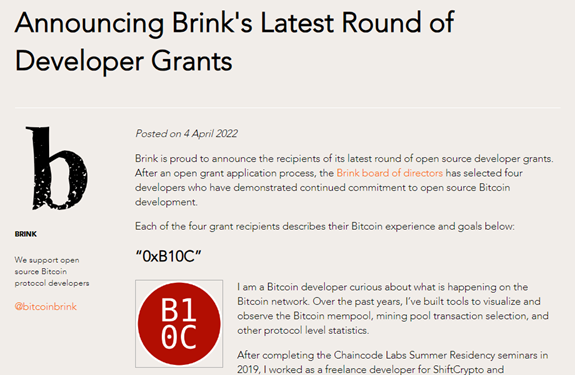
\includegraphics[width=0.72\textwidth]{figures/targeted_example.png}
    \caption{定向披露示例：Brink 官网受资助名单公告（2022年4月4日）}
    \label{fig:targeted-example}
\end{figure}

从期望理论的工具性维度分析，定向披露为非受助开发者提供了具体参照：他们能够看到哪类贡献者（以代码技能见长、常年深耕核心协议）最终获得了资助，由此推断自身活动与奖励之间的因果关联确实存在，进而形成”持续高质量参与便有机会进入下一轮资助名单”的工具性预期。该机制有别于非定向披露的效价驱动，它通过直接示范”绩效—奖励”路径来强化开发者的努力意愿。

但定向披露的排他性也具有两面性。名单公布的同时，绝大多数未入选者会意识到：这轮资助与自己无关。依据 Oliver（1980）\cite{oliver1980cognitive} 的期望失验理论，个体在行为结果与事先预期之间出现落差时，会产生情感负反应，并相应调整未来的期望水平。非受助开发者在非定向披露阶段形成的”可能成为受益者”的期望，将在定向披露的排他性公告面前遭受系统性的负向失验。这一心理机制预示着，定向披露可能反向削弱非定向披露对非受助开发者的后续激励效力。

\subsection{样本设计与识别策略}

准确识别捐赠信息披露的”纯信息效应”，是本研究面临的核心挑战。为此，样本设计层面进行了两项关键处理。

第一，剔除实际受助开发者。5次定向披露共涉及8名受助开发者，其活动行为受实质性货币激励驱动而非单纯信息刺激，纳入样本将使信息效应与货币效应发生混淆。本研究因此将上述8名开发者从分析样本中整体剔除，最终保留1,610名从未获得 Brink 资助的开发者。该设计确保所考察的激励效果来源于信息披露本身，而非实际发放的薪资奖励。

第二，选择个体固定效应框架。比特币核心开发者群体在经验积累、社区声誉、技术专长等维度上个体异质性显著，研究窗口期内的宏观市场环境（比特币价格波动、市场情绪周期）又构成共同的时间冲击。若不充分控制这两类系统性因素，估计结果将受到严重的遗漏变量偏误干扰。个体固定效应模型引入开发者个体固定效应（$u_i$）以吸收不随时间变化的个体异质性，同时纳入时间固定效应（$\lambda_t$）与丰富的时变控制变量（比特币市场表现、社区活跃度、Google Trends、项目进展），吸收时间维度的共同冲击，从而将分析聚焦于两类披露强度的随时间变动部分。

最终样本覆盖2022年第1周至2023年第52周共105个自然周、1,610名开发者，形成169,785个开发者—周面板观测单元，为因果推断提供充足的统计功效。

\section{研究假设}
\label{sec:hypotheses-1}

\subsection{非定向披露的正向主效应}

期望理论（Vroom, 1964）\cite{vroom1964work} 认为，个体的行为动机由效价、期望值与工具性三者的乘积共同决定。效价反映个体对预期奖励的主观价值判断——奖励对个体是否具有吸引力；期望值反映个体相信自身努力能转化为绩效的主观概率；工具性则反映个体相信绩效能换来奖励的主观概率。三个维度同时处于较高水平时，激励动力方可充分激活。

当 Brink 通过 X 平台公告披露一笔新收到的捐款时，该信息在比特币开发者社区中产生两方面信号效应。就效价而言，大额捐款的公开意味着 Brink 有能力为更多开发者提供实质性经济支持，奖励的吸引力由此得以强化。就期望值而言，稳定的资金流入表明资助项目具有持续性，开发者对”持续参与能带来未来回报”的信念因而得以巩固。两条心理路径共同作用，应会推动开发者在信息披露后短期内增加活动参与。

已有开源社区激励研究为上述逻辑提供了支持。Lakhani 和 Von Hippel（2004）\cite{lakhani2003open} 指出，开发者对潜在回报的预期是决定其投入水平的关键因素，外部资助信号明确时，内在驱动与外在激励相互叠加，产生”动机叠加”效应。Fang 和 Neufeld（2009）\cite{fang2009understanding} 对开源开发者持续参与行为的研究也发现，外部奖励预期的增强显著提升了开发者的参与意愿。B\'{e}nabou 和 Tirole（2003）\cite{benabou2003intrinsic} 的理论框架则表明，短期内信息型外部激励（如资助公告）能对内在动机产生补充性效果而非排挤效应，与非定向披露在激励方向上的预测一致。

上述推论在区分三类活动时仍然成立。代码活动（提交代码与发起 Pull Request）、审查活动（审查他人的 Pull Request）与讨论活动（参与 Issue 讨论）在认知投入程度和可见度上虽有差异，但同样受到期望激活机制的驱动。据此，本研究提出：

H1：非定向捐赠披露对开发者的整体开发者活动具有正向影响（H1a：代码活动；H1b：审查活动；H1c：讨论活动）。

\subsection{定向披露的正向主效应}

期望理论中的工具性维度关注一个核心判断：”绩效能否真正换来奖励？”非定向披露传递了资金充裕的信号，但并未明确回答”谁会获得资助”，仅提升了效价与期望值，却无法大幅增强开发者对工具性路径的确信。定向披露则通过公布受助名单，直接呈现”绩效—奖励”的真实案例，使非受助开发者得以对比受助者与自身特征，更准确地校准工具性预期。该信息的核心价值在于：将抽象的”有可能获得资助”的激励承诺转化为有据可查的参照路径。

信号理论（Spence, 1973; Connelly et al., 2011）\cite{spence1973job,connelly2011signaling} 为理解这一差异提供了框架。Brink 官方网站的受资助名单经严格筛选程序背书，属高可信度信号，其权威性高于 X 平台的即时公告。对开发者校准工具性预期而言，这一特性尤为关键——当一个可信赖机构正式宣告”谁通过了绩效评估并获得奖励”时，所传递的是关于”活动质量与资助资格之间关系”的最权威认证信息。Toubia 和 Stephen（2013）\cite{toubia2013intrinsic} 在社交媒体场景下的研究亦证实，信息源权威性较高时，个体对激励信号的响应强度随之增大。

定向披露还具有”榜样效应”的潜力。受助开发者的公开识别向社区传递了一种隐性规范：哪类深度参与（代码审查、持续提交高质量 Pull Request）会被识别和奖励。该规范信号有助于引导非受助开发者聚焦于类似的高质量活动方式，形成整体社区活动质量的正向外部性。Yang 等（2021）\cite{yang2021differential} 在开源社区持续参与研究中也指出，社会认可的可见度是影响开发者持续参与意愿的重要因素。据此，本研究提出：

H2：定向捐赠披露对开发者的整体开发者活动具有正向影响（H2a：代码活动；H2b：审查活动；H2c：讨论活动）。

\subsection{定向披露对非定向披露效应的负向调节}

定向披露本身虽对开发者活动有正向主效应，但它与非定向披露之间的交互关系却可能产生抑制效果。这一预判源自期望失验理论的核心命题（Oliver, 1980）\cite{oliver1980cognitive}：当个体实际结果低于事先形成的预期水平时，便产生负向失验，引发情感上的失望与认知层面的期望下修。该机制已在价格感知（Abrate et al., 2021）\cite{abrate2021relationship}、在线社区激励（Qiao et al., 2021）\cite{qiao2021mitigating}、用户生成内容平台（Sun et al., 2017）\cite{sun2017motivation} 等多个情景中获得实证验证。

在本研究情境中，失验机制的运作逻辑如下。每次非定向披露发布时，公告未指定受益方，社区中所有开发者均可合理推断自己未来有机会获得资助，由此形成弥漫性的”可能受益”期望状态，短期内活动参与随之增加。但一旦定向披露公布，明确的受助名单将绝大多数开发者排除在外。每轮仅有1至4名开发者获得资助，整个社区超过1600名开发者，未入选比例高达99\%以上——负向期望失验具有系统性和普遍性。

这种负向失验对开发者后续回应非定向披露的意愿将产生持续抑制，表现在两个层面。情感层面上，失望情绪降低了开发者对捐款公告积极信号的情感共鸣程度，使其无法充分调动对潜在奖励的期望动力。认知层面上，根据目标系统理论（Kruglanski et al., 2002）\cite{kruglanski2002theory}，当一个目标（获得 Brink 资助）的实现路径被事实性证伪后，个体会降低对该目标的期望权重，进而削减为此目标所付出的额外努力。两种抑制路径共同作用的结果是，定向披露发生后非定向披露的边际激励效应出现显著衰减。

从情绪信息理论（Schwarz \& Clore, 1983）\cite{schwarz1983moods} 的视角看，负向失验引发的消极情绪还会作为”背景感受”渗透到个体对未来激励信号的解读过程中——面对新的捐款公告时，开发者更倾向于以保守或中性态度加以评估，积极期望的激活程度由此降低。该情绪中介路径进一步强化了认知层面的抑制效果。据此，本研究提出：

H3：定向披露对非定向披露激励开发者活动的正向效应具有负向调节作用（H3a：代码活动；H3b：审查活动；H3c：讨论活动）。

综合以上三组假设，本研究的理论模型如图~\ref{fig:research-model-1} 所示。
图中将三组假设嵌入期望理论分析框架：
非定向披露经由效价路径（H1）提升开发者对资助的感知价值，
定向披露经由工具性路径（H2）强化"绩效可兑换资助"的信念，
两类披露的交互效应（H3）则体现为期望失验对激励动力的削弱。

\begin{figure}[htbp]
    \centering
    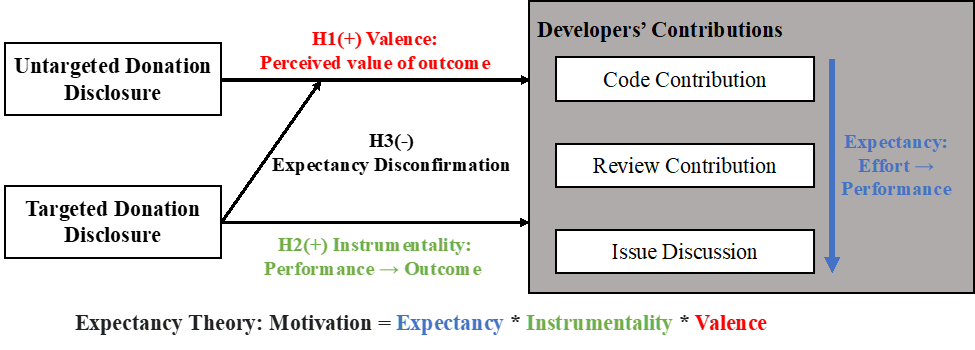
\includegraphics[width=0.72\textwidth]{figures/research_model_1.png}
    \caption{研究一理论假设模型（基于期望理论框架）}
    \label{fig:research-model-1}
\end{figure}

\section{数据与变量}
\label{sec:data-1}

\subsection{数据来源与样本构建}

本研究数据来源于多个公开平台，各类数据的来源、采集方式与粒度汇总于表~\ref{tab:data-source-1}。

\begin{table}[htbp]
    \centering
    \caption{研究一数据来源概览}
    \label{tab:data-source-1}
    \begin{tabularx}{\textwidth}{p{3cm}Xp{3cm}}
        \toprule
        数据类型 & 来源与说明 & 时间粒度 \\
        \midrule
        GitHub 开发活动
            & GH Archive（\url{https://www.gharchive.org}），
              包含 PushEvent（PE）、CreateEvent（CE）、DeleteEvent（DE）、CommitCommentEvent（CCE）、PullRequestEvent（PRE）、PullRequestReviewEvent（PRRE）、PullRequestReviewCommentEvent（PRRCE）、IssuesEvent（ISE）、IssueCommentEvent（ICE）九类事件
            & 小时 → 聚合至周 \\
        非定向披露事件
            & X 平台 @bitcoinbrink 官方账号，
              共采集19次捐款公告，
              15次含具体捐款金额（美元），
              其余仅披露捐款行为
            & 周 \\
        定向披露事件
            & Brink 官方网站受资助名单页面，
              人工标注各轮受助开发者姓名及公告日期，
              共5轮共计8名受助开发者
            & 事件 \\
        Bitcoin 市场数据
            & Yahoo Finance，
              抓取 BTC/USD 周收益率与周均交易量
            & 周 \\
        社会关注度（工具变量）
            & Google Trends，
              关键词 “Bitcoin Brink” 的周搜索量相对指数
            & 周 \\
        \bottomrule
    \end{tabularx}
\end{table}

样本构建方面，本研究以 2022 年 1 月第 1 周至 2023 年 12 月最后一周为观测窗口，共 105 个自然周。窗口选择基于如下考量：2022年1月是 Brink 完成初步组织运营并开始系统性发布捐款公告的起点，2023年12月为本研究数据可获得性的截止时点；两年观测期跨越多个 Bitcoin 市场周期（牛熊转换），保证了市场状态变化的足够异质性。

初始样本涵盖该期间内至少在 \texttt{bitcoin/bitcoin} 仓库产生过一次有效活动记录的所有开发者。以 GH Archive 的用户唯一标识符（login）为合并键，分别匹配 GitHub 开发活动、Brink 披露事件、Bitcoin 市场数据与 Google Trends 数据。合并过程以周为单位聚合：每位开发者每周的各类 GitHub 事件数量分别加总，得到开发者—周层面的面板数据集。

剔除上述 8 名实际受到 Brink 资助的开发者后，最终保留 1,610 名开发者，形成 $1{,}610 \times 105 = 169{,}050$ 个开发者—周面板观测单元。该完整面板反映了样本期内比特币核心社区开发者的持续参与特征。

\subsection{关键变量定义}

因变量设置为三类开发者活动指标，均经自然对数变换以缓解右偏分布问题。代码活动（$\ln\text{Code}_{it}$）定义为开发者 $i$ 在第 $t$ 周内代码提交相关事件数（包含 PE、CE、DE、CCE、PRE）的对数，反映主动推送代码的强度；审查活动（$\ln\text{Review}_{it}$）为代码审查相关事件数（PRRE、PRRCE）的对数，反映对他人代码的评审与质量把关行为；讨论活动（$\ln\text{Issue}_{it}$）为 Issue 提交事件数（ISE）的对数，反映参与社区技术讨论的广度。

非定向信息披露强度以 $UD_t$ 度量，操作化为第 $t$ 周及其前三周捐款金额四周移动平均值的自然对数。采用移动平均的理由是：捐款公告的信息传播和认知加工需要一定时间，移动平均能更准确地捕捉披露信息在社区中的累积扩散效应，而非仅关注当期瞬时冲击。定向信息披露以 $TD_t$ 度量，操作化为第 $t$ 周及其前三周公布的受资助开发者人数的四周移动平均值。相较于二值虚拟变量，该连续度量可区分不同批次定向披露的强度差异——例如2022年4月一次性公布4名受助者的信息冲击强度，显著高于此后每次仅公布1名受助者的情形。交互项 $UD_t \times TD_t$ 用于检验定向披露对非定向披露激励效果的调节作用。

模型纳入以下控制变量以尽可能吸收混淆因素。（1）比特币市场表现变量：比特币价格对数（$\text{lnClose}_t$）、交易量对数（$\text{lnVolume}_t$）和周收益率（$\text{Return}_t$），用以捕捉加密货币市场波动对开发者情绪与时间投入的影响。（2）开源社区活跃度变量：Fork 数对数（$\text{lnFork}_{it}$）和 Watch 数对数（$\text{lnWatch}_{it}$），反映开发者对比特币相关仓库的兴趣广度和社区整体关注度。（3）比特币 Google Trends 搜索指数对数（$\text{lnGtrend}_t$），控制比特币整体公众热度的时变趋势。（4）项目进展变量（$\text{Release}_t$），以 Bitcoin 核心仓库的 Release 事件衡量项目开发节奏，控制版本发布前后开发活动的自然波动。模型同时纳入时间固定效应（$\lambda_t$）以吸收各周共同的宏观冲击。

$Z_t$ 为”Bitcoin Brink”在第 $t$ 周的 Google Trends 搜索量指数四周移动平均值的对数，及其与定向披露的交互项 $Z_t \times TD_t$，分别作为 $UD_t$ 与交互项 $UD_t \times TD_t$ 的工具变量，详见第~\ref{sec:iv-method} 节的说明。

各变量定义汇总见表~\ref{tab:variables-1}。

\begin{table}[htbp]
    \centering
    \caption{研究一关键变量定义}
    \label{tab:variables-1}
    \begin{tabularx}{\textwidth}{p{4.2cm}p{1.8cm}X}
        \toprule
        变量 & 类型 & 定义 \\
        \midrule
        $\ln\text{Code}_{it}$ & 因变量 & 开发者 $i$ 在第 $t$ 周代码活动次数的对数（PE+CE+DE+CCE+PRE） \\
        $\ln\text{Review}_{it}$ & 因变量 & 开发者 $i$ 在第 $t$ 周审查活动次数的对数（PRRE+PRRCE） \\
        $\ln\text{Issue}_{it}$ & 因变量 & 开发者 $i$ 在第 $t$ 周讨论活动次数的对数（ISE） \\
        $UD_t$ & 核心自变量 & 非定向捐赠金额四周移动平均值的对数 \\
        $TD_t$ & 核心自变量 & 定向披露受资助人数的四周移动平均值 \\
        $UD_t \times TD_t$ & 交互项 & 非定向信息披露与定向信息披露的交互 \\
        $Z_t$ & 工具变量 & “Bitcoin Brink” Google Trends 四周移动平均值的对数 \\
        $\text{lnClose}_t$ & 控制变量 & Bitcoin 当周收盘价格的对数 \\
        $\text{lnVolume}_t$ & 控制变量 & Bitcoin 当周交易量的对数 \\
        $\text{Return}_t$ & 控制变量 & Bitcoin 当周价格收益率 \\
        $\text{lnFork}_{it}$ & 控制变量 & 开发者 Fork 数的对数，衡量社区活跃度 \\
        $\text{lnWatch}_{it}$ & 控制变量 & 开发者 Watch 数的对数，衡量社区关注度 \\
        $\text{lnGtrend}_t$ & 控制变量 & 比特币 Google Trends 搜索指数的对数 \\
        $\text{Release}_t$ & 控制变量 & Bitcoin 核心仓库当周 Release 事件数 \\
        \bottomrule
    \end{tabularx}
\end{table}

\subsection{描述性统计}

主要变量的描述性统计结果见表~\ref{tab:desc-stats}。就因变量而言，样本中开发者周均代码活动次数为 0.053（标准差 1.050），审查活动为 0.261（标准差 2.623），讨论活动为 0.014（标准差 0.279）。三类活动均值均远低于最大值（代码最高 71 次、审查最高 121 次、讨论最高 51 次），呈现典型右偏分布，反映开源社区中开发者活动强度的高度异质性。就核心自变量而言，非定向信息披露（$UD_t$）均值为 1.697（标准差 2.278），最大值为 7.429；由于该变量已取对数，零值表示当期及前三周均无捐款披露，最大值对应约 1,683 千美元的四周移动平均捐款金额。定向信息披露（$TD_t$）均值为 0.076（标准差 0.204），最大值为 1，反映受赠者公告属低频事件，但其随时间的变动为模型识别提供了必要的变异来源。工具变量（$Z_t$）均值为 71.816（标准差 8.305），变动范围为 59 至 90.172，为工具变量估计提供了足够的外生变动来源。

\begin{table}[htbp]
    \centering
    \caption{主要变量描述性统计（$N = 169{,}785$）}
    \label{tab:desc-stats}
    \begin{tabularx}{\textwidth}{Xrrrr}
        \toprule
        变量 & 均值 & 标准差 & 最小值 & 最大值 \\
        \midrule
        代码活动（$\text{Code}_{it}$）      & 0.053 & 1.050 & 0 & 71 \\
        审查活动（$\text{Review}_{it}$）    & 0.261 & 2.623 & 0 & 121 \\
        讨论活动（$\text{Issue}_{it}$）     & 0.014 & 0.279 & 0 & 51 \\
        非定向信息披露（$UD_t$） & 1.697 & 2.278 & 0 & 7.429 \\
        定向信息披露（$TD_t$） & 0.076 & 0.204 & 0 & 1 \\
        工具变量（$Z_t$） & 71.816 & 8.305 & 59 & 90.172 \\
        \bottomrule
    \end{tabularx}
\end{table}

描述性统计结果呈现若干规律。审查活动均值（0.261）显著高于代码活动均值（0.053）和讨论活动均值（0.014），说明在比特币核心开发生态中代码审查是开发者参与社区工作的主要形式，与开源社区”审查者多于提交者”的普遍特征相吻合；讨论活动均值最低，表明 Issue 参与在比特币核心项目中属相对低频的活动类型。非定向信息披露（$UD_t$）标准差（2.278）高于均值（1.697），反映 Brink 捐款披露在时间分布上波动较大——部分周期集中出现大额捐款公告，更多周期则为零披露。定向信息披露（$TD_t$）均值仅为 0.076，大多数周内并无新的受赠者公告，该变量的变动主要来源于公告发生前后的时间窗口。工具变量（$Z_t$）均值为 71.816、标准差为 8.305，”Bitcoin Brink”在 Google Trends 上的搜索热度整体较为稳定，但仍存在足够的时变波动，为识别捐款金额的外生变动提供了有效统计来源。

为进一步考察关键变量间的相关关系，本研究计算了主要变量的 Pearson 相关系数矩阵（表~\ref{tab:correlation}）。

\begin{table}[htbp]
    \centering
    \caption{主要变量相关系数矩阵}
    \label{tab:correlation}
    \small
    \begin{tabularx}{\textwidth}{Xrrrrrr}
        \toprule
        & 代码活动 & 审查活动 & 讨论活动 & $UD$ & $TD$ & $Z$ \\
        \midrule
        代码活动（Code）     & 1.000 & & & & & \\
        审查活动（Review）   & 0.462 & 1.000 & & & & \\
        讨论活动（Issue）    & 0.576 & 0.285 & 1.000 & & & \\
        非定向信息披露（$UD$）  & 0.000 & $-$0.002 & $-$0.001 & 1.000 & & \\
        定向信息披露（$TD$）    & 0.006 & 0.009 & 0.005 & 0.025 & 1.000 & \\
        工具变量（$Z$）        & 0.005 & 0.009 & 0.001 & 0.200 & 0.222 & 1.000 \\
        \bottomrule
    \end{tabularx}
    \begin{minipage}{\textwidth}
        \vspace{0.3em}
        \footnotesize 注：N=169,785（个体-周观测值）。
        Code：代码活动次数（PE+CE+DE+CCE+PRE）；Review：审查活动次数（PRRE+PRRCE）；Issue：讨论活动次数（ISE）；
        $UD$：非定向信息披露（四周移动平均捐款金额的对数）；$TD$：定向信息披露（四周移动平均受赠者人数）；$Z$：工具变量（Google Trends 四周移动平均指数的对数）。
        各变量间相关系数均低于 0.6，不存在严重的多重共线性问题。
    \end{minipage}
\end{table}

相关系数矩阵揭示了几方面信息。第一，三类开发者活动之间存在中等程度正相关（Code-Review: 0.462；Code-Issue: 0.576；Review-Issue: 0.285），但均未超过 0.6 阈值，说明活跃开发者在不同类型活动上的投入正向关联，支持将三类活动纳入同一分析框架的合理性，同时三者各自保持了足够的独立变异。第二，非定向信息披露（$UD$）与各类活动的相关系数均接近零（0.000至$-$0.002），截面层面尚未显示显著的描述性关联，这与自变量通过面板回归在时间维度上识别因果效应的策略相吻合。第三，工具变量（$Z$）与非定向信息披露（$UD$）的相关系数为 0.200，与定向信息披露（$TD$）的相关系数为 0.222，表明公众搜索关注度同 Brink 捐赠及资助活动正相关，初步支持工具变量的相关性条件；$Z$ 与三类开发者活动的相关系数均极低（0.001至0.009），初步佐证了排他性约束的合理性。第四，所有变量间相关系数均低于 0.6，模型不存在严重的多重共线性问题。

\section{计量模型}
\label{sec:model-1}

\subsection{基准个体固定效应模型}
\label{sec:fe-model}

本研究以双向固定效应面板模型为基准估计框架，纳入个体固定效应与时间固定效应，并辅以丰富的时变控制变量（比特币市场变量、社区活跃度变量、Google Trends、项目进展变量）吸收时间维度的共同冲击。具体设定如下：

\begin{equation}
\label{eq:fe-model}
Y_{it} = \beta_1 UD_t + \beta_2 TD_t
       + \beta_3 (UD_t \times TD_t)
       + \boldsymbol{\gamma}' \mathbf{X}_{it} + u_i + \lambda_t + \varepsilon_{it}
\end{equation}

其中，$Y_{it}$ 为开发者 $i$ 在第 $t$ 周的某类开发者活动数量（$\text{Code}_{it}$、$\text{Review}_{it}$ 或 $\text{Issue}_{it}$）；$UD_t$ 为非定向信息披露强度，操作化为四周移动平均捐赠金额的对数；$TD_t$ 为定向信息披露强度，操作化为四周移动平均受赠者公告人数；$UD_t \times TD_t$ 为两者的交互项，用于检验定向披露对非定向披露效应的调节作用；$\mathbf{X}_{it}$ 为控制变量向量，包括比特币市场表现变量（$\text{lnClose}_t$、$\text{lnVolume}_t$、$\text{Return}_t$）、开源社区活跃度变量（$\text{lnFork}_{it}$、$\text{lnWatch}_{it}$）、比特币 Google Trends（$\text{lnGtrend}_t$）、项目进展变量（$\text{Release}_t$）；$u_i$ 为个体固定效应，吸收开发者层面的不随时间变化的特征（如技术背景、偏好、性格）；$\lambda_t$ 为时间固定效应，吸收各周共同的宏观冲击（如市场周期、政策事件等）；$\varepsilon_{it}$ 为残差项。本研究采用四周移动平均对核心自变量进行平滑处理，以减轻单周数据波动的噪声，更好地捕捉信息披露效应的渐进传导过程。

核心参数的预期符号为：$\beta_1 > 0$（H1）、$\beta_2 > 0$（H2）、$\beta_3 < 0$（H3）。直觉上，$\beta_3 < 0$ 意味着当定向披露强度增大（$TD_t$ 取值越高）时，非定向披露的边际激励系数从 $\beta_1$ 下降至 $\beta_1 + \beta_3 \cdot TD_t$，定向披露的频次越高，非定向披露激励效应的衰减幅度越大。

该设定的识别假设是：控制个体效应和丰富时变控制变量后，捐款披露金额的随时间变动部分与个体层面未观测异质性不相关。非定向披露本质上由外部捐赠方行为触发，属偶发性事件，其时间分布在相当程度上具有外生性；个体固定效应的引入进一步剔除了开发者内生选择的影响。

极端观测值的处理方面，因变量为计数型数据且分布高度右偏（如表~\ref{tab:desc-stats} 所示，代码活动最大值达59次、审查活动最大值达121次），本研究对所有因变量实施标准 Winsorize 处理（第1百分位和第99百分位为截断点），降低极端值对参数估计稳定性的影响。为解决面板数据中常见的序列相关与截面相关问题，估计过程采用双向聚类标准误（clustered by developer and week），以确保统计推断的有效性。

\subsection{工具变量方法（2SLS）}
\label{sec:iv-method}

固定效应模型虽已在很大程度上控制了可观测和部分不可观测的混淆因素，捐款金额变量仍可能存在内生性问题。一个潜在的反向因果路径如下：比特币核心开发社区活跃度较高时，项目市场可见度和公众关注度随之提升，可能吸引更多外部捐赠方向 Brink 发起捐款，进而增大非定向披露金额。若此机制存在，$UD_t$ 与误差项 $\varepsilon_{it}$ 之间存在正相关，FE 估计量对 $\beta_1$ 的估计将出现正向偏误。交互项 $UD_t \times TD_t$ 包含内生的 $UD_t$ 成分，同样需进行内生性处理。

为此，本研究采用两阶段最小二乘法（2SLS）处理内生性问题。模型中有两个内生变量——$UD_t$（非定向信息披露强度）和 $UD_t \times TD_t$（交互项），对应构建两个工具变量：（1）$Z_t$，即”Bitcoin Brink”Google Trends 搜索指数的四周移动平均值取对数，作为非定向披露强度的工具变量；（2）$Z_t \times TD_t$，即搜索指数与定向披露的交互项，作为 $UD_t \times TD_t$ 的工具变量。工具变量的合理性论证如下。相关性方面：公众对 Brink 的搜索兴趣升高时，往往意味着 Brink 知名度和品牌曝光度处于高峰，机构或个人捐赠方更有可能发起大额捐款，搜索指数与捐款金额之间因而存在显著正相关。排他性方面：Google 搜索指数反映的是互联网用户的信息查询行为，该行为本身不会直接影响特定开发者某一周内的 GitHub 活动次数——开发者的代码产出主要由技术任务进度、个人时间安排与社区内部协作节奏决定，而非外部公众的搜索行为，排他性约束具有合理的理论支撑。

2SLS 的两阶段设定如下：

\begin{align}
\text{（第一阶段）}\quad
    \widehat{UD}_t
        &= \alpha_0 + \alpha_1 Z_t
           + \alpha_2 Z_t \times TD_t
           + \alpha_3 TD_t
           + \boldsymbol{\alpha}' \mathbf{X}_{it} + u_i + \eta_{it}
\label{eq:first-stage} \\[0.5em]
    \widehat{UD \times TD}_t
        &= \delta_0 + \delta_1 Z_t
           + \delta_2 Z_t \times TD_t
           + \delta_3 TD_t
           + \boldsymbol{\delta}' \mathbf{X}_{it} + u_i + \xi_{it}
\label{eq:first-stage-2} \\[0.5em]
\text{（第二阶段）}\quad
    Y_{it}
        &= \beta_1 \widehat{UD}_t
           + \beta_2 TD_t
           + \beta_3 \widehat{UD \times TD}_t
           + \boldsymbol{\gamma}' \mathbf{X}_{it}
           + u_i + \varepsilon_{it}
\label{eq:second-stage}
\end{align}

在第一阶段方程~\eqref{eq:first-stage} 和~\eqref{eq:first-stage-2} 中，两个工具变量分别被用于预测非定向披露强度及其与定向披露的交互项的外生变动部分；第二阶段方程~\eqref{eq:second-stage} 以第一阶段的拟合值替代内生变量进行估计，从而剔除与误差项相关的内生成分。工具变量的有效性通过 Anderson 识别检验（欠识别检验）和 Cragg-Donald Wald F 统计量（弱工具变量检验）加以验证。

\section{实证结果}
\label{sec:results-1}

\subsection{主效应分析}

表~\ref{tab:main-results} 报告了固定效应（FE）模型和工具变量（2SLS）模型的主要估计结果，因变量分别为代码活动、审查活动与讨论活动。

\begin{table}[htbp]
    \centering
    \caption{捐赠信息披露对开发者活动的影响：主回归结果}
    \label{tab:main-results}
    \small
    \begin{tabularx}{\textwidth}{Xrrrrrr}
        \toprule
        & \multicolumn{3}{c}{固定效应模型（FE）}
        & \multicolumn{3}{c}{工具变量模型（2SLS）} \\
        \cmidrule(lr){2-4}\cmidrule(lr){5-7}
        变量
            & 代码活动 & 审查活动 & 讨论活动
            & 代码活动 & 审查活动 & 讨论活动 \\
        \midrule
        非定向信息披露（$UD_t$）
            & 0.000$^{**}$  & 0.001$^{**}$  & $-$0.000
            & 0.003$^{***}$ & 0.008$^{***}$ & 0.000 \\
            & (2.36)        & (2.06)        & ($-$0.00)
            & (3.12)        & (3.14)        & (0.45) \\[0.4em]
        定向信息披露（$TD_t$）
            & 0.005$^{**}$  & 0.017$^{***}$ & 0.000
            & 0.061$^{***}$ & 0.198$^{***}$ & 0.011 \\
            & (2.54)        & (3.46)        & (0.03)
            & (2.74)        & (2.98)        & (0.88) \\[0.4em]
        交互项（$UD_t \times TD_t$）
            & $-$0.001      & $-$0.001      & 0.001$^{*}$
            & $-$0.041$^{**}$ & $-$0.133$^{***}$ & $-$0.007 \\
            & ($-$1.13)     & ($-$0.94)     & (1.83)
            & ($-$2.56)     & ($-$2.78)     & ($-$0.79) \\[0.4em]
        \midrule
        个体固定效应 & 是 & 是 & 是 & 是 & 是 & 是 \\
        时间固定效应 & 是 & 是 & 是 & 是 & 是 & 是 \\
        控制变量     & 是 & 是 & 是 & 是 & 是 & 是 \\
        \midrule
        $N$         & 169,050 & 169,050 & 169,050 & 169,050 & 169,050 & 169,050 \\
        $N_g$       & 1,610   & 1,610   & 1,610   & 1,610   & 1,610   & 1,610 \\
        $F$         & 10.986  & 6.926   & 7.423   & 11.041  & 7.176   & 7.185 \\
        Adj. $R^2$  & 0.007   & 0.002   & 0.003   & $-$0.041 & $-$0.088 & $-$0.010 \\
        Anderson LM 检验    & --- & --- & --- & \multicolumn{3}{c}{1609.515$^{***}$} \\
        Cragg-Donald F 统计量 & --- & --- & --- & \multicolumn{3}{c}{2,790,000} \\
        \bottomrule
    \end{tabularx}
    \begin{minipage}{\textwidth}
        \vspace{0.3em}
        \footnotesize 注：括号内为 $t$ 统计量；$^{*}p<0.1$，$^{**}p<0.05$，$^{***}p<0.01$。
        控制变量包括比特币价格（lnClose）、交易量（lnVolume）、收益率（Return）、Fork 数（lnFork）、Watch 数（lnWatch）、Google Trends（lnGtrend）、项目进展（Release）；模型同时控制个体固定效应与时间固定效应。
        Anderson LM 检验与 Cragg-Donald F 统计量对三类因变量一致，此处合并报告。
    \end{minipage}
\end{table}

固定效应模型中，非定向信息披露（$UD_t$）系数在代码活动上显著为正（$\beta_1 = 0.000$，$t = 2.36$，$p < 0.05$），审查活动上同样显著为正（$\beta_1 = 0.001$，$t = 2.06$，$p < 0.05$），讨论活动上系数接近零且不显著（$t = -0.00$）。经 2SLS 估计后，代码活动和审查活动的系数幅度均明显扩大（分别为 0.003 和 0.008），显著性水平提升至 1\%，说明修正内生性偏误后非定向披露的正向激励效果更为突出。H1a 和 H1b 得到支持，H1c 未获统计证据。从期望理论框架来看（参见图~\ref{fig:research-model-1}），这一结果可由期望值维度加以解释。期望值反映的是开发者对"努力$\to$绩效"关联的主观估计：代码提交和代码审查属可直接观测的技术产出，与获得资助方认可和奖励之间有清晰的绩效关联；讨论活动（如提交 Issue）更多体现为社区协商行为，对绩效认定乃至资助的贡献路径较为间接。当捐赠信息披露激活开发者对奖励的预期时，增量努力倾向于分配到期望值较高的代码与审查活动上，讨论活动的响应因而不显著。

定向信息披露（$TD_t$）的系数在固定效应模型中，代码活动（$\beta_2 = 0.005$，$t = 2.54$，$p < 0.05$）和审查活动（$\beta_2 = 0.017$，$t = 3.46$，$p < 0.01$）均显著为正，讨论活动上不显著。2SLS 模型中，代码活动和审查活动系数分别升至 0.061 和 0.198，均在 1\% 水平显著，与 FE 结果方向一致且更为稳健。H2a 与 H2b 获得支持，H2c 未获显著证据。该模式与 H1 的发现相互印证：定向披露通过揭示”绩效$\to$奖励”路径进一步强化了工具性感知，但这种强化同样集中于绩效关联明确的代码与审查活动，对讨论活动的期望值提升有限。需指出的是，定向披露在本模型中以连续变量（四周移动平均受赠者人数）而非虚拟变量刻画，其系数的经济含义为：受赠者公告数量每增加一人，对开发者审查活动的边际激励效应为 0.017（FE）或 0.198（2SLS）。

交互项（$UD_t \times TD_t$）系数在 FE 模型中对代码活动（$\beta_3 = -0.001$，$t = -1.13$）和审查活动（$\beta_3 = -0.001$，$t = -0.94$）方向为负但统计上不显著。但在 2SLS 模型中，交互项系数显著增大：代码活动为 $-0.041$（$t = -2.56$，$p < 0.05$），审查活动为 $-0.133$（$t = -2.78$，$p < 0.01$），均达到统计显著水平。FE 模型中交互项不显著而 2SLS 模型中显著，这一差异恰恰反映了内生性偏误的影响——FE 模型未处理非定向披露的内生性，交互项的调节效应被衰减偏误所掩盖；2SLS 模型通过工具变量剔除捐款金额的内生成分后，定向披露对非定向披露的负向调节作用方得以真实呈现。以审查活动为例：当 $TD_t = 1$（即近期每周均有一名受赠者公告）时，非定向披露净效应为 $\beta_1 + \beta_3 = 0.008 - 0.133 = -0.125$，表明高频率定向披露不仅抵消了非定向披露的正向激励，甚至使其转为负向效应。H3a 和 H3b 在 2SLS 模型中获得支持，H3c 未达显著水平。

Anderson LM 检验统计量为 1609.515（$p < 0.001$），拒绝”工具变量不足以识别”的零假设，两个工具变量具有足够的联合识别力。Cragg-Donald Wald F 统计量为 $2.79 \times 10^6$，远超 Stock-Yogo（2005）\cite{stock2005testing}弱工具变量检验临界值，排除了弱工具变量的可能性。第一阶段回归中，$Z_t$ 对 $UD_t$ 的系数为 7.461（$t = 8348.74$，$p < 0.01$），预测能力极强，进一步佐证了工具变量的相关性条件。综合以上检验结果，本研究所用工具变量满足相关性与排他性要求，2SLS 估计结果具备可信的因果解释基础。

\subsection{结果解读与经济意义}

以审查活动为例讨论结果的经济意义。2SLS 模型中，非定向信息披露每增加 1\%（即对数变动 $\Delta UD = 0.01$），在无定向披露（$TD_t = 0$）条件下，开发者周均审查活动次数增加约 $0.008 \times 0.01 = 0.00008$ 次。相对于样本均值（0.261 次/周），这相当于约 0.035\% 的边际提升。该数字看似微小，但对于具有高度社会溢出效应的基础设施代码审查而言，极小比例的活动增量聚合到1610人社区后，意味着每周额外产生约 0.13 次审查事件，年化超过 6 次额外的核心代码审查——对提升比特币协议安全性具有实质价值。

从另一角度审视效应量级：Brink 观测期内最大一次捐款（500万美元）对数值约为 15.42，与均值（约 3.87，基于有捐款记录的周次）差距约 11.55 个单位。换言之，相较于一次普通规模的捐款公告，一次500万美元大额公告在无定向披露条件下将额外带来约 $0.008 \times 11.55 \approx 0.092$ 次的开发者周均审查活动；聚合到1610名开发者，相当于整个社区额外增加约 148 次审查事件。对于通常每月仅有数百次高质量审查的比特币核心仓库，这一量级的社区激励价值不可忽视。

就定向披露的调节效应而言，当其强度增大时（如 $TD_t = 0.5$，即近期平均每两周有一名受赠者被公告），非定向披露对审查活动的净边际效应为 $\beta_1 + \beta_3 \times 0.5 = 0.008 - 0.133 \times 0.5 = -0.059$（2SLS 模型），捐款公告的激励效果不仅完全消失，甚至出现明显负向效应。这意味着，在定向披露较为频繁的时期，Brink 持续发布的捐款公告从激励角度看不仅无效，反而可能产生反向效果。该发现对后续捐款公告的传播策略调整具有直接的政策含义。

\section{稳健性检验}
\label{sec:robust-1}

为检验基准结果的稳健性，本研究对核心自变量的度量方式做了三组替代性处理，分别从变量形式（连续值 vs. 虚拟变量）和时间平滑方式（移动平均 vs. 当期值）两个维度加以变换。结果汇总于表~\ref{tab:robustness-all}。

\subsection{稳健性检验一：虚拟变量形式与时间窗口（$-1, 2$）}

基准模型以连续值的四周移动平均形式度量两类信息披露变量。但开发者对信息的响应未必呈线性——他们可能仅对”有无披露事件”做出反应，而对具体金额大小不敏感。第一组稳健性检验因此将非定向披露和定向披露均替换为虚拟变量形式，并设置（$-1, 2$）时间窗口：事件发生前一周至后两周窗口内取1，否则取0。该设定既考虑信息传播的滞后效应，也纳入了可能存在的预期效应。

结果显示，非定向披露虚拟变量在代码活动上系数为 0.005（$t = 2.75$，$p < 0.01$），审查活动上为 0.013（$t = 2.18$，$p < 0.05$），均显著为正。定向披露虚拟变量在代码活动上为 0.004（$t = 2.78$，$p < 0.01$），审查活动上为 0.019（$t = 4.64$，$p < 0.01$），同样显著为正。交互项在代码活动（$-0.009$，$t = -3.52$，$p < 0.01$）和审查活动（$-0.033$，$t = -4.90$，$p < 0.01$）上均显著为负。以上表明，即便以二值度量替代连续变量并采用不同时间窗口设定，主要结论仍然成立。

\subsection{稳健性检验二：连续值形式与当期度量}

第二组检验保留连续值形式，但去除四周移动平均处理，直接使用当期（第 $t$ 周）的捐款金额对数和受赠者公告人数。目的在于考察基准模型中移动平均平滑处理是否实质性地改变了估计结果——主效应究竟来源于当期信息冲击，还是移动平均带来的时序扩散。

结果显示，当期非定向披露在代码活动上系数为 0.002（$t = 3.71$，$p < 0.01$），审查活动上为 0.007（$t = 3.37$，$p < 0.01$），均在 1\% 水平显著。交互项在代码活动（$-0.001$，$t = -2.82$，$p < 0.01$）和审查活动（$-0.004$，$t = -2.62$，$p < 0.01$）上同样显著为负。与基准模型相比，当期度量系数量级有所变化，但符号和显著性完全一致，确认移动平均处理并未人为制造统计显著性。

\subsection{稳健性检验三：虚拟变量形式与当期度量}

第三组检验将两类信息披露变量均替换为当期虚拟变量（有披露取1，无披露取0），不做时间窗口扩展。这是最为保守的度量方式，仅考虑披露事件发生当周的即时效应。

结果显示，非定向披露虚拟变量在代码活动上系数为 0.015（$t = 3.63$，$p < 0.01$），审查活动上为 0.045（$t = 3.36$，$p < 0.01$），效应量级较移动平均形式有所放大但方向一致。交互项在代码活动（$-0.014$，$t = -3.63$，$p < 0.01$）和审查活动（$-0.040$，$t = -3.19$，$p < 0.01$）上均高度显著为负。定向披露虚拟变量在代码活动和审查活动上系数分别为 0.003（$t = 2.21$，$p < 0.05$）和 0.008（$t = 2.19$，$p < 0.05$），与基准模型方向一致。

\begin{table}[htbp]
    \centering
    \caption{稳健性检验：不同变量形式与度量方式下的估计结果}
    \label{tab:robustness-all}
    \small
    \begin{tabularx}{\textwidth}{Xrrrrrr}
        \toprule
        & \multicolumn{2}{c}{检验一：虚拟变量+窗口}
        & \multicolumn{2}{c}{检验二：连续值+当期}
        & \multicolumn{2}{c}{检验三：虚拟变量+当期} \\
        \cmidrule(lr){2-3}\cmidrule(lr){4-5}\cmidrule(lr){6-7}
        变量 & 代码 & 审查 & 代码 & 审查 & 代码 & 审查 \\
        \midrule
        非定向信息披露（$UD_t$）
            & 0.005$^{***}$ & 0.013$^{**}$
            & 0.002$^{***}$ & 0.007$^{***}$
            & 0.015$^{***}$ & 0.045$^{***}$ \\
            & (2.75) & (2.18)
            & (3.71) & (3.37)
            & (3.63) & (3.36) \\[0.4em]
        定向信息披露（$TD_t$）
            & 0.004$^{***}$ & 0.019$^{***}$
            & 0.001$^{**}$ & 0.002
            & 0.003$^{**}$ & 0.008$^{**}$ \\
            & (2.78) & (4.64)
            & (2.09) & (1.64)
            & (2.21) & (2.19) \\[0.4em]
        交互项（$UD_t \times TD_t$）
            & $-$0.009$^{***}$ & $-$0.033$^{***}$
            & $-$0.001$^{***}$ & $-$0.004$^{***}$
            & $-$0.014$^{***}$ & $-$0.040$^{***}$ \\
            & ($-$3.52) & ($-$4.90)
            & ($-$2.82) & ($-$2.62)
            & ($-$3.63) & ($-$3.19) \\[0.4em]
        \midrule
        控制变量 & 是 & 是 & 是 & 是 & 是 & 是 \\
        个体固定效应 & 是 & 是 & 是 & 是 & 是 & 是 \\
        $N$ & 169,050 & 169,050 & 169,050 & 169,050 & 169,050 & 169,050 \\
        \bottomrule
    \end{tabularx}
    \begin{minipage}{\textwidth}
        \vspace{0.3em}
        \footnotesize 注：括号内为 $t$ 统计量；$^{*}p<0.1$，$^{**}p<0.05$，$^{***}p<0.01$。
        检验一：非定向和定向披露均为虚拟变量，时间窗口为（$-1, 2$）；
        检验二：非定向披露为当期捐款金额对数，定向披露为当期受赠者公告人数；
        检验三：非定向和定向披露均为当期虚拟变量（有/无事件）。
        所有模型均包含与基准模型相同的控制变量。
    \end{minipage}
\end{table}

综合三组检验，不论将核心自变量从连续值变换为虚拟变量，还是从四周移动平均变换为当期度量，亦或设置不同时间窗口，主要结论均保持高度一致：非定向披露对代码活动和审查活动有显著正向主效应（H1），定向披露同样有正向主效应（H2），两者交互项显著为负（H3）。三组检验中讨论活动系数均不显著，与基准模型发现一致。这些结果表明核心发现不依赖于特定变量度量方式或时间平滑处理的选择，稳健性良好。

\section{机制分析}
\label{sec:mechanism-1}

主效应分析揭示了捐赠信息披露对开发者活动的平均处理效应，但该效应在不同类型开发者间是否存在显著差异，是检验理论机制的关键所在。本研究设计两组异质性检验：将样本按特定维度划分为高低两组并分别进行 2SLS 估计，检验各组系数是否存在统计上的显著差异。这种分组回归方法（亦称”调节分析”）能揭示信息激励的作用边界——何种特征下激励效果更强或更弱，从而为期望理论与期望失验理论的机制解释提供更精细的证据。

两个分析维度的选择遵循如下理论逻辑。（1）比特币项目投入程度反映开发者对比特币核心项目的历史开发活动水平，是”项目嵌入深度”的直接度量。（2）开源社区活跃程度以开发者个人仓库数量衡量其在更广泛开源生态中的参与广度，是”开源社区整体嵌入程度”的代理变量。两个维度分别从项目深度和社区广度刻画开发者的嵌入关系，为验证”高嵌入度开发者对信息激励更为敏感”这一理论预测提供多维证据基础。

\subsection{比特币项目投入程度的异质性：重度投入者与轻度投入者}

根据开发者在比特币项目中的开发活动量，以中位数为分界点将样本划分为重度投入者（总活动量高于中位数，$N = 97{,}335$，$N_g = 927$）和轻度投入者（总活动量低于或等于中位数，$N = 71{,}715$，$N_g = 683$），分别在两个子样本上重新估计 2SLS 模型。表~\ref{tab:mechanism-heavy-light} 报告了两组的估计结果。

\begin{table}[htbp]
    \centering
    \caption{机制分析：比特币项目投入程度的异质性}
    \label{tab:mechanism-heavy-light}
    \small
    \begin{tabularx}{\textwidth}{Xrrrrrr}
        \toprule
        & \multicolumn{3}{c}{重度投入者}
        & \multicolumn{3}{c}{轻度投入者} \\
        \cmidrule(lr){2-4}\cmidrule(lr){5-7}
        变量 & 代码 & 审查 & 讨论 & 代码 & 审查 & 讨论 \\
        \midrule
        非定向信息披露（$UD_t$）
            & 0.004$^{***}$ & 0.014$^{***}$ & 0.001
            & 0.000 & $-$0.000 & $-$0.001 \\
            & (2.92) & (3.15) & (0.95)
            & (1.39) & ($-$0.11) & ($-$1.27) \\[0.4em]
        定向信息披露（$TD_t$）
            & 0.099$^{***}$ & 0.345$^{***}$ & 0.026
            & 0.010 & $-$0.000 & $-$0.009 \\
            & (2.60) & (2.99) & (1.25)
            & (1.08) & ($-$0.07) & ($-$0.85) \\[0.4em]
        交互项（$UD_t \times TD_t$）
            & $-$0.067$^{**}$ & $-$0.231$^{***}$ & $-$0.018
            & $-$0.007 & 0.000 & 0.007 \\
            & ($-$2.42) & ($-$2.79) & ($-$1.19)
            & ($-$1.05) & (0.09) & (0.92) \\[0.4em]
        \midrule
        个体固定效应 & 是 & 是 & 是 & 是 & 是 & 是 \\
        控制变量 & 是 & 是 & 是 & 是 & 是 & 是 \\
        $N$ & 97,335 & 97,335 & 97,335 & 71,715 & 71,715 & 71,715 \\
        \bottomrule
    \end{tabularx}
    \begin{minipage}{\textwidth}
        \vspace{0.3em}
        \footnotesize 注：括号内为 $t$ 统计量；$^{*}p<0.1$，$^{**}p<0.05$，$^{***}p<0.01$。
        按开发者在比特币项目开发活动的中位数划分。
    \end{minipage}
\end{table}

结果显示，重度投入者的非定向披露系数在代码活动上为 0.004（$t = 2.92$，$p < 0.01$），审查活动上为 0.014（$t = 3.15$，$p < 0.01$），均显著为正且量级约为全样本平均效应的两倍；轻度投入者对应系数在三类活动上均未达到统计显著水平。定向披露效应同样呈现鲜明分化：重度投入者的定向披露系数在审查活动上高达 0.345（$t = 2.99$，$p < 0.01$），轻度投入者则接近零。这一异质性结果有清晰的理论解释——期望理论的激励效果对已深度嵌入项目、长期积极参与的开发者更为显著，原因在于他们对捐赠信号的解读更为准确，对”绩效可转化为奖励”的评估更为乐观；轻度投入者因缺乏足够社区知识或历史活动积累，难以将捐款信号转化为自身受益的期望，对信息披露的响应相对迟钝。交互项系数在重度投入者中对代码活动（$-0.067$，$p < 0.05$）和审查活动（$-0.231$，$p < 0.01$）均显著为负，轻度投入者中则不显著，进一步说明期望失验机制主要作用于与激励系统深度关联的积极参与者。

\subsection{开源社区活跃程度的异质性：开源活跃者与开源非活跃者}

第二个维度以开发者个人仓库数量衡量其在更广泛开源社区中的活跃程度，以中位数为界划分为开源活跃者（个人仓库数高于中位数，$N = 86{,}100$，$N_g = 820$）和开源非活跃者（个人仓库数低于或等于中位数，$N = 82{,}950$，$N_g = 790$），分别进行 2SLS 估计。该分组与比特币项目投入程度分析存在交叉但并非等同：项目投入度衡量的是开发者在比特币特定项目中的深度，开源活跃度反映的则是其在整个开源生态中的参与广度。两个维度共同刻画”社区嵌入程度”的不同侧面。

\begin{table}[htbp]
    \centering
    \caption{机制分析：开源社区活跃程度的异质性}
    \label{tab:mechanism-active}
    \small
    \begin{tabularx}{\textwidth}{Xrrrrrr}
        \toprule
        & \multicolumn{3}{c}{开源活跃者}
        & \multicolumn{3}{c}{开源非活跃者} \\
        \cmidrule(lr){2-4}\cmidrule(lr){5-7}
        变量 & 代码 & 审查 & 讨论 & 代码 & 审查 & 讨论 \\
        \midrule
        非定向信息披露（$UD_t$）
            & 0.004$^{***}$ & 0.016$^{***}$ & 0.001
            & 0.001 & $-$0.001 & $-$0.000 \\
            & (2.68) & (3.56) & (1.04)
            & (1.54) & ($-$0.56) & ($-$0.85) \\[0.4em]
        定向信息披露（$TD_t$）
            & 0.105$^{**}$ & 0.426$^{***}$ & 0.033
            & 0.013 & $-$0.039 & $-$0.012 \\
            & (2.54) & (3.49) & (1.52)
            & (0.83) & ($-$0.83) & ($-$0.84) \\[0.4em]
        交互项（$UD_t \times TD_t$）
            & $-$0.072$^{**}$ & $-$0.291$^{***}$ & $-$0.024
            & $-$0.007 & 0.032 & 0.010 \\
            & ($-$2.40) & ($-$3.32) & ($-$1.51)
            & ($-$0.67) & (0.94) & (0.97) \\[0.4em]
        \midrule
        个体固定效应 & 是 & 是 & 是 & 是 & 是 & 是 \\
        控制变量 & 是 & 是 & 是 & 是 & 是 & 是 \\
        $N$ & 86,100 & 86,100 & 86,100 & 82,950 & 82,950 & 82,950 \\
        \bottomrule
    \end{tabularx}
    \begin{minipage}{\textwidth}
        \vspace{0.3em}
        \footnotesize 注：括号内为 $t$ 统计量；$^{*}p<0.1$，$^{**}p<0.05$，$^{***}p<0.01$。
        按开发者个人仓库数量的中位数划分。
    \end{minipage}
\end{table}

结果与比特币项目投入度异质性分析高度吻合。开源活跃者的非定向披露系数在代码活动上为 0.004（$t = 2.68$，$p < 0.01$），审查活动上为 0.016（$t = 3.56$，$p < 0.01$），三项假设的系数在代码和审查活动上均显著；开源非活跃者的所有核心系数则均无统计显著性。这表明捐赠信息披露的激励效应具有明显的”存量依赖性”——唯有在开源社区中保持广泛参与的开发者，才会将捐款信息纳入活动决策的考量框架。开源参与较少的开发者，Brink 信息披露并不在其日常关注范围之内，激励效应无从产生。交互项系数在开源活跃者中对代码活动（$-0.072$，$p < 0.05$）和审查活动（$-0.291$，$p < 0.01$）均高度显著为负，开源非活跃者中则不显著甚至方向相反。这一鲜明分化再次印证：期望失验机制主要作用于深度嵌入社区的活跃开发者群体。

两组分析结论高度一致，共同指向一个核心发现：捐赠信息披露的激励效应在很大程度上取决于开发者与社区之间的嵌入程度。无论以比特币项目投入深度还是开源社区参与广度衡量，嵌入程度更高的开发者不仅从非定向披露中获得更多正向激励，也在定向披露频率增大时经历更明显的期望失验，最终导致更强的负向调节效应。这种”双重敏感性”揭示了期望机制在活跃开发者群体中的放大效应，为理解开源社区中激励分配不均衡性提供了新的理论线索。

综合两组异质性分析可见，信息型激励的效果并非在所有开发者中均匀分布，而是呈现强烈的”核心群体主导”特征。这一发现对开源社区资助策略设计有重要意义：资助机构若希望通过信息披露整体激活社区活力，策略上应特别关注如何触达和激励活跃核心群体，因为边缘参与者对信息激励相对不敏感。与此同时，核心开发者群体因高度嵌入社区而对失验效应更为脆弱，定向披露的频率与时序设计尤需审慎，以免对这批社区中流砥柱造成不必要的期望透支。

\section{本章小结}
\label{sec:summary-1}

本章聚焦 Bitcoin Brink 基金会两种捐赠信息披露方式（非定向披露与定向披露）对比特币开源社区开发者活动的影响。综合运用个体固定效应模型与两阶段最小二乘法，基于 2022 年至 2023 年间 169,785 个开发者—周面板观测（1,610 名开发者），对三组假设进行了系统检验。

研究场景上，本章以 Bitcoin Brink 生态为准自然实验场景，其两阶段信息披露结构（X 平台捐款公告 + 官网受资助名单）提供了清晰的识别机会。通过剔除实际受助开发者，分析被锁定在信息披露的纯信息激励效应上，有效排除了实际货币奖励的干扰。有别于既有研究，本章将定向披露从二值虚拟变量扩展为连续度量（四周移动平均受赠者人数），更精细地捕捉了定向披露强度的边际效应。

假设验证方面，主要发现可概括为三点。第一，非定向披露对代码活动和审查活动有显著正向主效应（H1a、H1b 成立），捐款规模信号能通过激活期望理论中的效价与期望值维度有效促进开发者技术活动，但对讨论活动影响不显著。第二，定向披露对代码活动和审查活动同样有显著正向主效应（H2a、H2b 成立），受资助名单的公布通过提供”绩效—奖励”的可观察因果链强化了非受助开发者的工具性动机。第三，定向披露频率增大会显著削弱非定向披露对代码和审查活动的激励效应（H3a、H3b 在 2SLS 模型中成立）；交互项系数在 FE 模型中方向为负但不显著，在 2SLS 模型中则达到统计显著水平——这一差异恰恰反映了内生性偏误对调节效应的衰减作用。负向调节效应与期望失验理论的预测高度吻合：定向披露频率越高，未入选者经历的期望失验越强烈，对后续非定向披露信号的响应敏感度越低。

机制检验上，两组异质性分析（比特币项目重度/轻度投入者、开源社区活跃者/非活跃者）均指向共同结论：信息激励效应高度集中于深度嵌入社区的活跃开发者群体。重度投入者的非定向披露系数在审查活动上为 0.014（$p < 0.01$），开源活跃者为 0.016（$p < 0.01$），均约为全样本均值的两倍。投入较少、参与不活跃的开发者群体中三类假设均无法获得显著支持，表明捐赠信息披露的激励杠杆在核心群体与边缘参与者之间存在显著的作用分化。

方法稳健性上，三组替代性度量检验（虚拟变量加时间窗口$(-1, 2)$、连续值当期度量、虚拟变量当期度量）均证实主要结论可靠，核心变量符号和显著性在不同度量方式下保持高度一致。工具变量有效性检验（Anderson LM 统计量 1609.515，Cragg-Donald F 统计量 $2.79 \times 10^6$）确认了 2SLS 策略的合理性，排除了内生性偏误对主要结论的威胁。

本章的理论贡献体现在以下几个层面。

第一，理论框架上，本章将期望理论（Vroom, 1964）\cite{vroom1964work} 与期望失验理论（Oliver, 1980）\cite{oliver1980cognitive} 整合为统一解释两类披露效果的分析框架。既有文献对这两个理论多为单独应用：期望理论主要用于解释激励信号的正向驱动机制，期望失验理论主要用于解释满意度的形成。本章通过识别非定向披露（激活期望）与定向披露（诱发失验）之间的动态交互关系，在开源社区激励情境中首次将两者加以整合，揭示”信息型正向激励”与”信息型负向调节”的共存条件及相互作用机制。

第二，研究情境上，本章以比特币开源社区与 Bitcoin Brink 基金会为场景，利用双阶段披露结构（非定向的 X 平台公告与定向的官网名单）构建了准自然实验设计。该设计的优越性在于：两类披露行为的发生时序均由外部因素（捐赠方行为与基金会审核流程）决定，具有相当程度的外生性；样本中排除实际受助开发者，确保分析聚焦于纯信息效应。这一设计为后续类似情境的研究提供了可供参照的方法论范式。

第三，方法论上，本章采用个体固定效应与工具变量相结合的识别策略，构建两个工具变量（Google Trends 搜索指数及其与定向披露的交互项）处理两个内生变量（非定向披露强度及其与定向披露的交互项），并通过多重稳健性检验和机制分析增强结论的可信度。

实践层面，本章发现对比特币核心开发社区的生态治理及更广泛的开源资助机构均有重要启示。第一，非定向披露是一种低成本、普惠性的激励工具，在定向披露频率较低时社区激励效果显著；资助机构应善用 X 平台等公开渠道，保持捐款信息的及时透明披露，持续激活社区开发者的参与热情。第二，定向披露虽能正向激励非受助开发者（通过工具性预期机制），但频率增大所引发的期望失验效应会系统性削弱非定向披露的激励价值。资助机构发布受助名单时应合理控制公告频率，并同步配合期望管理措施——如强调资助名额将持续扩大、明确下一轮评选周期等——以缓解负向失验效应的累积影响。第三，机制分析揭示信息型激励效果高度集中于活跃且深度嵌入社区的核心开发者群体。对边缘参与者而言，单纯的捐款信息披露难以有效激活其参与意愿；资助机构若希望扩大激励覆盖面，还需辅以更具针对性的参与引导机制（如导师制度、新人资助项目、开发任务清单等）。

综上，本章从实证角度揭示了开源社区捐赠信息披露的双重激励效应，为理解开源社区中信息激励机制提供了新的理论视角和经验证据，也为后续章节中社区讨论情感效应的研究奠定了比较基础。两类影响因素共同构成本研究对比特币开发者行为决定机制的完整图景。


%%====================================================================
